\documentclass[11pt,twoside,a4paper]{article}
\usepackage[english]{babel} %English hyphenation
\usepackage{amsmath} %Mathematical stuff
\usepackage{amsthm}
\usepackage{amssymb}
\usepackage{graphicx}

%Hyperreferences in the document. (e.g. \ref is clickable)
\usepackage{hyperref}

%Pseudocode
\usepackage{algorithm}
\usepackage[noend]{algpseudocode}
%You can also use the pseudocode package. http://cacr.uwaterloo.ca/~dstinson/papers/pseudocode.pdf
%\usepackage{pseudocode}

\usepackage{a4wide,times}
\title{TI2736-C Assignment 1} 
\author{
	Joost Pluim, jwpluim, 4162269 \\
	Pascal Remeijsen, premeijsen, 4286243
}
\begin{document}
\maketitle
\clearpage

\chapter{Perceptron}

\section{Question 0}
	
	\subsection{Question 0.1}
	The new formula to determine if the threshold is reached is
	
	\begin{equation}
		(w')^T x' \geq 0
	\end{equation}
	
	\subsection{Question 0.2}
	By multiplying the transposed vector with vector $x'$ and checking if the result is positive or negative. Both positive and negative represent a class by which the feature vector can be evaluated. 
				
\section{Question 2}

	\subsection{Question 2.1}
	If the learning rate is low, the weights vector is only changed very little in every iteration and therefore will converge slowly and may converge to local optimum.\\
	If the learning rate is high, the weights vector is changed a lot for every faulty training record. This means the weights factor will oscillate a lot and can therefore easily oversee the real optimum.
	
\section{Question 3}

	\subsection{Question 3.1}
	The yellow line represents the weights-vector. If we want to know the prediction of a label, we just multiply the (x,y) by the weights-vector. \\
	Therefore the black line, which is the decision boundary, represents all points for which $w' x^{T}' = 0$. This means that the decision boundary is the inverse of the weights vector.  
	
\begin{figure}[ht]
    \centering
    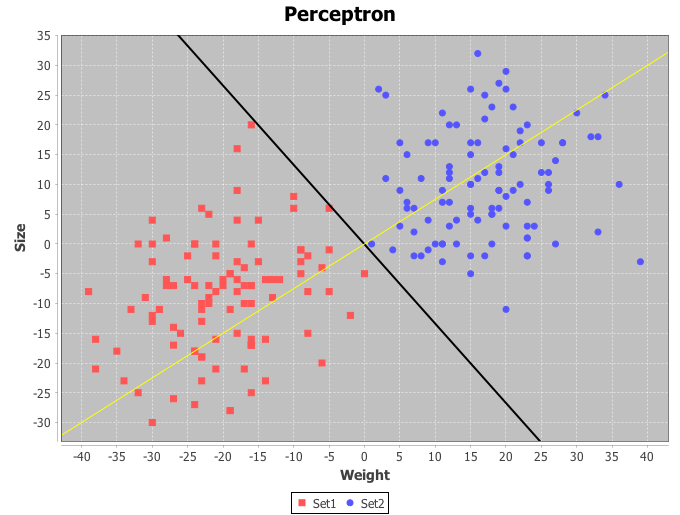
\includegraphics[width=\textwidth]{perceptron.png}
    \caption{The decision boundary (in black) and weights vector (in yellow)}
\end{figure}
	
	\subsection{Question 3.2}
	Call the decision boundary $D$, then:
	
	\begin{equation}
		D = (w')^{-1}
	\end{equation}
	
\section{Question 4}

	\subsection{Question 4.1}
	The dataset contains 100 images from which 50 belong to one classification and 50 belong to the other classification. In the dataset the feature-vector is represented by all numbers after the first number because the first number represents the label. \\
	The first 50 records represent handwritten zeros represented by label -1, the last 50 records are handwritten ones, represented by the label 1.
	
\section{Question 6}

	\subsection{Question 6.1}
	We know that ones are represented by a positive label, zeros by a negative label. This means that if a certain input is multiplied with the weights-vector, the output should become negative for a zero, and positive for a one. \\
	In the image, the grey parts represent parts which don't influence the outcome very much. Black parts represent parts which are important for the zeros and are weights which are big negative weights. White parts are the parts which are important for the ones, and therefore are big positive weights. 
	
\begin{figure}[ht]
    \centering
    
\includegraphics[scale=0.5]{digits_weights.png}
    \caption{Visualisation of the weights after two iterations of training.}
\end{figure}	
	
\section{Question 7}

	\subsection{Question 7.1}
	If we run our training algorithm multiple times on our training data it will probably (if possible) assign exactly those weights so that the prediction with these weights would be perfect for all points in our training set. \\
	Therefore we need a completely different set of data points which isn\'t taken into account in our training, to test our $w$ for errors and make sure we don\'t overfit our weights vector.
	
\section{Question 8}

	\subsection{Question 8.1}
	From the 400 test records, 6 are misclassified. From these 1 is a one which is located a little bit too far to the left and has big base and tilting top. The zeros don\'t have a very big gap in the middle. All 6 records are quite different than most other inputs and are therefore misclassified.

\chapter{Nearest Neighbour}

\section{Question 1}

	\subsection{Question 1.1}
	If $k$ is set to 3 and we have the three points as described in the exercise, the predicted label would be the $b$, since they are with two and the point with class $a$, which is way closer, is only with 1. \\
	We could fix this by setting our $k$ lower, or when determining the label, taking into account the distance from the input point to prevent the two points which are second and third closest, however are really far away, from deciding the label.
	
\section{Question 3}

	\subsection{Question 3.1}
	The NN-classifier is slightly slower than the perceptron approach, since we have to sort our data. If we compare the error rate with the perceptron approach, we see it is way smaller, which votes for the NN approach.  

		
	
\begin{thebibliography}{9}
\end{thebibliography}
\end{document}
